\documentclass[journal]{IEEEtran}

% *** OPTIONAL PACKAGES ***
\usepackage{cite}
\usepackage[pdftex]{graphicx}
\usepackage[cmex10]{amsmath}

\usepackage[utf8]{inputenc}
%\usepackage{algorithmic}
%\usepackage{array}
%\usepackage[caption=false,font=footnotesize]{subfig}
%\usepackage{fixltx2e}
%\usepackage{stfloats}
%\usepackage{url}
%\usepackage{hyperref}

% correct bad hyphenation here
\hyphenation{op-tical net-works semi-conduc-tor}

\begin{document}

\title{Robô Recepcionista \\
	Pioneer P5-DX}

\author{\large Pioneer 5 \normalsize \\
Pedro Isidro - 67220,
~Diogo Silva - 75136,
~João Pedrosa - 79833}

% The paper headers
\markboth{Sistemas Autónomos - 2013/2014 - 1\textsuperscript{o} Semestre}{Instituto Superior Técnico}

% make the title area
\maketitle

\begin{abstract}
Abstract (summary of the work)
\end{abstract}

% Note that keywords are not normally used for peerreview papers.
\begin{IEEEkeywords}
Pioneer P5-DX, ROS, autónomo.
\end{IEEEkeywords}

\section{Introdução}
% start with \IEEEPARstart{first letter}{rest of first word}
%Introduction and Motivation (brief description of what the project was about and the motivation for the topic)

Os requisitos para do nosso projecto exigiam ter um robô Pioneer P3-DX capaz de executar tarefas modeladas por uma máquina de estados finitos. Essas tarefas incluem o robô ser capaz de mapear, auto-localiza-se e navegar o seu ambiente e deslocar-se para diferentes localizações indicadas através de interação com utilizadores.

A nossa motivação foi ter um robô recepcionista capaz de receber visitantes num edifício, e.g. um bloco de escritórios. O robô seria capaz de mapear o edifício \emph{a priori} para futura utilização, de receber um conjunto de coordenadas já conhecidas (e.g. escritórios de certas pessoas) associadas a palavras-chave, de interagir com utilizadores através de síntese e reconhecimento de voz e, por fim, de guiar os mesmos aos seus destinos.

Durante a implementação do projecto simplificámos algumas destas funcionalidades, nomeadamente o mapeamento e o reconhecimento de voz. O mapeamento foi executado apenas no quinto piso da Torre Norte do IST. O reconhecimento de voz foi restringido a um pequenos dicionário para reduzir a complexidade e a necessidade de adaptar modelos acústicos e treinamento.

%The requirements for our project were having a Pioneer P3-DX capable of carrying out tasks modeled through a Finite State Automaton consisting of mapping, self-localizing and navigating its environment and move to different locations indicated by user interaction.

%Our motivation was to have a receptionist robot, capable of greeting visitors in a big building such as an office block. The robot would be capable of mapping the building \emph{a priori}, receive a set of known coordinates such as people's offices associated with keywords, interact with users through speech synthesis and voice recognition and  guide visitors to their desired destinations.

%During the implementation of the project we simplified on some of these functionalaties, e.g. mapping only the fifth floor of the IST's North Tower and the voice commands were only single word phrases - mostly numbers.

\hfill December 6, 2013

\section{Algoritmos e Implementação}
%Methods and Algorithms (brief explanation of the methods used and ROS packages/algorithms used - this is mainly to make sure you understood the conceptual and the implementation part, and to introduce notation - do not write like in a book or tutorial paper)

\subsection{Mapeamento}
%gmapping - mapping and SLAM using odometry
%
%map\_server - save map and serve map

O mapeamento é um problema complexo pois involve a estimação simultânea da posição do robô e do mapa em seu redor. Os dados recebidos de odometria vão ser utilizados para estimar a posição $x$. Utilizando a posição $x$ e os dados do laser $z$ po

\begin{eqnarray}
  \label{eq:map_1}
  d = \{ z_1,...,z_n \} \\
  \hat{m} = arg_m max \{ P(m|d) \}
\end{eqnarray}

onde $\hat{m}$ é o mapa mais provável. Os dados da odometria são utilizados para estimar a posição $x$ do robô no mapa, que é uma grelha de ocupação.

	To do the Mapping of 5 floor, we use the gmapping.
	\\
	\\
	Hokuyo node:
	\\
	The Hokuyo node obtain the data of Hokuyo connected to the computer and
	publishe in topic scan.
	\\

	Gmapping:
	\\
	The gmapping get the information in topics tf and scan. The topic tf transforms necessary to relate frames for laser, base, and odometry. The topic scan transforms Laser scans to create the map from.
	The gmapping give the topic map for creating the map.
	\\


	Initial Map creating in gmapping
	\begin{figure}[ht]
	\centering
	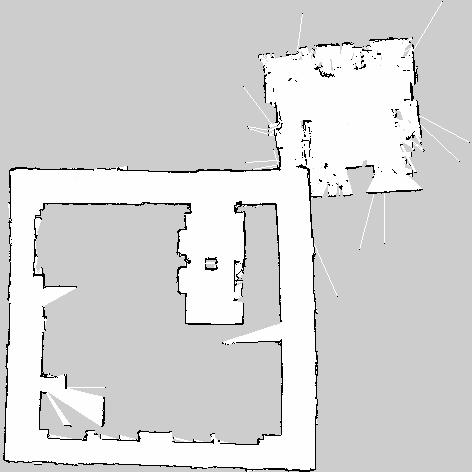
\includegraphics[width=21pc]{map.jpeg}
	\caption{Initial Map}
	\label{fig_env}
	\end{figure}
	\\

\subsection{Localização}

%amcl - localization
%
%RosAria - metapackage with odometry package, communication with robot
%
%hokuyo\_node - laser ranger

\subsection{Navegação}

%navigation stack - navigation
% - move\_base
% - local planner
% - global planner

	For doing the Navigation the used commands gived by the user
	\\
	\\
	Odometry:
	\\
	\\
	The pose have tree parameters: x, y , $\theta$




	Algorithm:







	We use Rosaria to obtain odometry information for doing the localization in the map, the odometry information obtain in topic pose published by Rosaria.
	Another thing we use Rosaria is for reading the sonar, give by the topic sonar.
	\\
	\\

\subsection{Execução do Plano Coordenado}

Para conseguir coordenar as acções do robô de maneira a executar a tarefa proposta, é necessário ter uma representação abstracta dessa mesma tarefa. O robô recepcionista é um sistema sequencial, ou seja, executa uma acção de cada vez -- ou mover-se para uma posição-alvo ou interagir com o utilizador para adquirir esse objectivo. Para tais sistemas, o fluxo de controlo é usualmente especificado recorrendo a uma Máquina de Estados Finitos (MEF).
Uma MEF é então implementada no nó \textit{p3dx\_smach}, usando o pacote \textit{smach}. A tarefa do robô é dividida em três estados de execução: INITIAL, TO\_GOAL e GET\_GOAL. A Figura~\ref{fig: maquina_estados}, gerada pelo nó \textit{smach\_viewer}, ilustra a forma como o controlo flui entre os estados. De seguida explica-se o funcionamento de cada estado.

\begin{figure}[ht]
	\centering
	\includegraphics[height=7cm]{state_machine}
	\caption{Fluxo de execução da máquina de estados.}
	\label{fig: maquina_estados}
\end{figure}

\subsubsection{INITIAL} Estado inicial. O nó verifica se os ficheiros relativos ao mapa (\textit{.pmg} e \textit{.yaml}) estão presentes e lê o ficheiro de texto com as especificações dos diferentes locais de interesse (\textit{setpoints}), guardando-os num dicionário. Caso ocorra alguma erro neste processo , retorna-se \textit{error} e a execução é interrompida. Caso contrário, restorna-se \textit{ready} e o controlo é passado ao estado \textit{TO\_GOAL}, com instruções para levar o robô até à base. Neste projecto, a posição base é em frente aos elevadores. Numa aplicação geral, esta seria, por exemplo, a entrada de um edifício.

\subsubsection{TO\_GOAL} Este estado recebe como argumento do estado anterior o identificador da posiçao-alvo. De seguida procura esse identificador no dicionário de \textit{setpoints} para obter as coordenadas e orientação correspondentes. Por último, uma ordem é enviada para o nó de navegação \textit{move\_base}, usando um cliente de acção criado com o pacote \textit{actionlib}. O servidor de acção encontra-se já implementado na \textit{stack} de navegação, pelo nó \textit{move\_base\_msgs}. O controlo é mantido até que o objectivo seja alcançado ou cancelado pelo utilizador, sendo então passado para o estado \textit{GET\_GOAL}, com vista a determinar a próxima directiva. São também passados argumentos que indicam qual foi o objectivo perseguido e se este foi alcançado ou cancelado. Mais uma vez, caso ocorra algum erro no processo, como o robô se perca ou o caminho se encontre bloqueado, este estado retorna \textit{error} e a execução é interrompida.

\subsubsection{GET\_GOAL} À excepção do primeiro objectivo, que é invariavelmente a base, as posições alvo têm de ser determinadas pro interacção com o utilizador. \textit{GET\_GOAL} encarrega-se dessa tarefa, recorrendo aos nós de reconhecimento de fala (\textit{pocketsphinx}) e de síntese de voz (\textit{say}). Caso o robô se encontre na base -- o que pode ser determinado pelos argumentos fornecidos por \textit{TO\_GOAL} -- o robô simplesmente aguarda que um utilizador inicie a interacção, voltando a executar o mesmo estado se nenhum objectivo for transmitido. Caso contrário, o pŕoprio robô pede ao utilizador um novo objectivo, ordenando o retorno à base se este recusar ou o ignorar durante um certo período de tempo.


\subsection{Interacção com o utilizador}

A interacção com utilizadores foi feita com recurso a reconhecimento e síntese de voz. Para o primeiro, foram testados duas soluções com características muito distintas. Para o último, foi utilizado um síntetizador de som com capacidade de síntetizar voz a partir de um texto recebido.

\subsubsection{Reconhecimento de voz}

Para compreender como é que o reconhecimento de voz é realizado é necessário introduzir alguns conceitos importantes. A unidade básica da fala é entendida como um \emph{fone}. Contudo, as características acústicas correspondentes a um fone variam conforme o contexto em que esse fone aparece, a pessoa, etc. Devido a estas variações  utilizam-se subestados dentro de um fone para melhorar o reconhecimento. Usa-se, também, o contexto em que os fones aparecem, o que se irá traduzir num problema de procura do contexto que melhor se aproxima dos dados recebidos. Os fones constróem sílabas. Dependendo das condições de fala, a mesma sílaba correponde a diferenes fones. Palavras restringem considerávelmente a quantidade de fones que se têm de comparar e quanto menor for o dicionário mais rápido será o reconhecimento.

Uma das soluções testadas foi a livraria \textit{Pocketsphinx} da plataforma Sphinx. Esta livraria, disponível num pacote do ROS com o mesmo nome, está optimizada para portabilidade que é exactamente o que pretendemos na implementação num robô. A plataforma Sphinx utiliza algoritmos extensivamente utilizados em investigação baseados em \textit{Hidden Markov Models} (HMM). Os principais componentes do processo de reconhecimento de voz esão representados na Figura \ref{fig:voicerecprocess}.

\begin{figure}[ht]
  \centering
  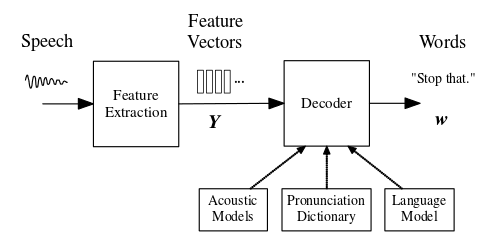
\includegraphics[width=21pc]{voice_rec_process.png}
  \caption{Principais componentes do processo de reconhecimento de fala.}
  \label{fig:voicerecprocess}
\end{figure}

O audio recebido pelo microfone é convertido em numa sequência de vectores acústicos $Y_{1:T}=y_1,...,y_T$, num processo denominado de extração de \textit{features}. Os números dos vectores são baseados nas propriedades acústicas da fração correspondente na sequência. Depois desta extração, o descodificador tenta encontrar a sequência de palavras $w_{1:L}=w_1,...,w_L$ que é mais provável ter estado na origem de $Y$, ou seja:

%fix equation
\begin{equation}
\label{eq:word_bestmatch}
  \hat{w}=arg_w max \{ P(w|Y) \}
\end{equation}

No entanto, $P(w|Y)$ é difícil de modelar directamente, pelo que se utiliza a regra de Bayes para transformar (\ref{eq:word_bestmatch})
 no equivalente:

\begin{eqnarray}
  \label{eq:word_bestmatch_equi}
   \hat{w} = arg_w max \{ p(Y|w) P(w) \}
\end{eqnarray}

A verossimilhança $p(Y|w)$ é determinada pelo \emph{modelo acústico} e a probabilidade $P(w)$ é determinada pelo \emph{modelo de linguagem}. Para qualquer palavra $w$, é criado um modelo acústico pela concatenação de modelos fonéticos para criar palavras como elas são definidas num dicionário de pronunciação. Os modelos fonéticos podem ser treinados especificamente para dicionários, ambientes ou contextos específicos. O modelo de lingagem é um modelo em que a probabilidade da palavra $N$ é dependente apenas nos seus $N-1$ antecessores. Os parâmetros no modelo de línguagem são determinados através da contagem da ocorrência das palavras no $corpus$ do texto.

%O reconhecimento é feito a partir de uma amostra que é separada em diferentes partes por silêncios ou pausas e depois tenta-se identificar o que é dito em cada uma dessas partes comparando com todas as combinações de palavras. O resultado é a melhor combinação possível. Esta comparação tem em conta três conceitos importantes. O primeiro é o de \textit{features} - a fala é dividida em pequenas partes (frações de segundo) e de cada parte é exradido um conjunto de números designado por vector de \textit{features}. O segundo é o modelo utilizado - objecto matemático que codifica propriedades da fala, normalmento baseado no especto. Por último, é o processo de procura em si, que pode ser mais ou menos simplificado para devolver resultados em tempos com utilização prática. A forma como o vector de \textit{features} é calculado, o quão o modelo utilizado se aproxima da realidade e o uso ou não de simplificações ou optimizações do processo de procura vão influenciar a qualidade do reconhecimento de fala.

Assim, para o reconhecimento de voz é feito pelo nó \textit{pocketsphinx}, recebendo como argumentos um dicionário de pronunciações e um modelo de linguagem. Para o nosso projecto modificámos o código original para também aceitar outros modelos acústicos que não o original. Desta forma, podemos carregar um modelo que melhor se adapte à nossa utilização.

Apesar de não o termos feito, o desempenho do reconhecimento de voz poderia ter sido melhorado se se tivesse treinado o modelo acústico ou adaptado ao dicionário utilizado.

%A outra solução testada foi um \textit{wraper} do \emph{Google Speech API}. Esta solução tem a grande vantagem de nos dar acesso a uma plataforma poderosa de reconhecimento de voz. O pacote utilizado foi o \textit{gspeech} que grava uma amostra de audio em formato \emph{FLAC} durante um período de tempo, envia-a para os servidores da Google, recebe a resposta e publica o resultado e o grau de cereza do reconhecimento de voz.

\subsubsection{Síntese de voz}

A síntese de voz foi feita com recurso ao pacote \textit{sound\_play} da \textit{stack} \textit{audio\_common}. O algoritmo trata qualquer som (ficheiro \emph{WAV} ou \emph{OGG} ou texto sintetisado) como algo que pode ser reproduzido ou parado. O estado da reprodução de um som pode ser mudado através da publicação para um tópico específico \textit{robotsound}. O nó \textit{soundplay\_node} é o nó responsável pela reprodução do som. Os restantes nós do pacote servem para fornecer o som a ser reproduzido. O nó que nos dá acesso à síntese de voz é o \textit{say} que recebe texto por argumento da linha de comandos ou de um texto. O código deste nó foi alterado por forma a receber texto por subscrição a um tópico. A síntese de voz é feita através do \emph{Festival}.


\subsection{Visualização}

%Rviz - visualization

The project was developed on the Robot Operating System framework, which is open-source and contains a myriad of different off-the-shelf packages ready for use.

\section{Resultados}
% Experimental Results (show the most relevant results to illustrate the merits and the possible unresoved issues)


\subsection{Reconhecimento de voz}
\label{sec:resuts_recvoice}

Tendo em conta a nossa utilização do robô como recepcionista, o dicionário de pronunciações foi limitado a um pequeno número de palavras. Foram introduzidas algumas palavras de comandos para o robô e as restantes estavam associadas a localizações. Os modelos acústico e fonético utilizados estão adaptados apenas para utilização com língua Inglesa, pelo que os comandos e nomes de localizações escolhidos foram, de igual forma, em língua Inglesa.

O microfone utilizado foi o imbutido num Os resultados que obtivemos foram bastante satisfatórios num ambiente com pouco ruido, mesmo com a utilização de um modelo acústico não adaptado. As palavras \textit{hello}, \textit{yes} e \textit{no} foram quase sempre reconhecidas à primeira e raramente mal intrepretadas por outras palavras. Os nomes das localizações eram mais frequentemente confundidos com outras palavras, mas geralmente não com nomes de outras localizações, pelo que não afectava muito o desempenho do sistema.

\subsection{Síntese de voz}
\label{sec:results_sintvoice}

Os nós da síntese de voz reproduziram com sucesso as frases enviadas. O discurso, apesar de não natural como o discurso humano, foi perceptível e compreensível. As frases síntetizadas foram \textit{``hello''} quando o robô iniciava ou estava na base, \textit{``where to go''} depois do utilizador expressar intenção em ser guiado pelo robô, \textit{``repeat please''} quando o robô não percebia o que era dito ou não encontrava correspondente nas localizações guardadas, \textit{``want to go anywhere else''} quando o robô chega a um destino que não a base e \textit{``goal was canceled''} quando um objectivo é cancelado.



\section{Conclusão}
% Conclusions (lessons taken, major conclusions, reasons for what went wrong, if anything)


\appendices
% if have a single appendix:
%\appendix[Proof of the Zonklar Equations]
% or
%\appendix  % for no appendix heading
\section{Title of Appendix A}
Appendix A text goes here.
desired:

\begin{thebibliography}{1}
\bibitem{IEEEhowto:kopka}
	H.~Kopka and P.~W. Daly, \emph{A Guide to \LaTeX}, 3rd~ed.\hskip 1em plus
	0.5em minus 0.4em\relax Harlow, England: Addison-Wesley, 1999.
\end{thebibliography}

\end{document}

%----------------------------

% Floating figure
\begin{figure}[!t]
\centering
\includegraphics[width=2.5in]{myfigure}
\caption{Simulation Results.}
\label{fig_sim}
\end{figure}

% Double column floating figure using two subfigures.
\begin{figure*}[!t]
\centering
\subfloat[Case I]{\includegraphics[width=2.5in]{box}%
\label{fig_first_case}}
\hfil
\subfloat[Case II]{\includegraphics[width=2.5in]{box}%
\label{fig_second_case}}
\caption{Simulation results.}
\label{fig_sim}
\end{figure*}

% Floating table
\begin{table}[!t]
% increase table row spacing, adjust to taste
\renewcommand{\arraystretch}{1.3}
 if using array.sty, it might be a good idea to tweak the value of
 \extrarowheight as needed to properly center the text within the cells
\caption{An Example of a Table}
\label{table_example}
\centering
% Some packages, such as MDW tools, offer better commands for making tables
% than the plain LaTeX2e tabular which is used here.
\begin{tabular}{|c||c|}
\hline
One & Two\\
\hline
Three & Four\\
\hline
\end{tabular}
\end{table}
